\documentclass[professionalfont, 12pt, handout, t]{beamer} %, handout



%\usepackage{pxfonts}
%\usepackage{eulervm}

%\documentclass[sans,mathserif]{beamer}
%\usepackage{kerkis} % Kerkis roman and sans
%\usepackage{kmath}


%\documentclass[serif, professionalfont]{beamer} %
%\usepackage[T1]{fontenc} % Needed for Type1 Concrete
%\usepackage{concrete}

%\usepackage[Chinese]{babel}
%\usepackage[T1]{fontenc}

\usepackage{amsmath}
\usepackage{amsthm}
\usepackage{amsthm,amssymb,amsfonts,amsmath} 
\usepackage{proof}
\usepackage[mathscr]{eucal}
\usepackage{amssymb,mathtools}
\usepackage{xcolor}
\usepackage{mathrsfs}
\usepackage{enumerate}
\usepackage{comment}
\usepackage{pifont}
\usepackage{caption}

\usepackage{graphicx}
\graphicspath{{./Geometry}{./Geometry Solution 1}{./Geometry Solution 2}}
\usepackage{caption}

\usepackage{tikz}
\usetikzlibrary{shapes.geometric}
\usetikzlibrary{arrows}
\usetikzlibrary{shapes}
\usetikzlibrary{plotmarks}

\theoremstyle{plain}
\newtheorem{thm}{Theorem}
\newtheorem{remark}{Remark}
\newtheorem{cor}[thm]{Corollary}
 
\theoremstyle{definition}
\newtheorem{df}{Definition}
       
  
\usepackage{epsfig}
%\usepackage{amsmath}
%\usepackage{mathrsfs}
%\usepackage[all]{xy}  
%\usepackage{proof}    %%proof.style file
           

\newcommand{\tcb}[1]{\textcolor{blue}{#1}}
\newcommand{\tcr}[1]{\textcolor{red}{#1}}  
\newcommand{\tcc}[1]{\textcolor{cyan}{#1}}
\newcommand{\tcg}[1]{\textcolor{green}{#1}} 
\newcommand{\tcm}[1]{\textcolor{magenta}{#1}}      

\newcommand{\omt}{\mathop{\curlywedge}}
    
\newcommand{\Lra}{\: \Leftrightarrow \:}
\newcommand{\m}[1]{{\mathbf {#1} }}
%\newcommand{\m}[1]{{\mbox{\uppercase {\bf {#1}}}}}
%\newcommand{\N}[1]{{{ \m N_{#1}}}}
\newcommand{\Rl}{ {\mbox{$\mathcal{RL}  $}}}
\newcommand{\Rlc}{ {\mbox{$\mathcal{RL}^C  $}}}
\newcommand{\Ra}{{ \:\; \Rightarrow \:\; }}
%\newcommand{\Ra}{{\mbox{$ \: \Rightarrow \: $}}}
\newcommand{\Rar}{{ \: \Rightarrow \: }}
\newcommand{\La}{{\mbox{$ \: \Leftarrow \: $}}}
\newcommand{\ra}{\rightarrow}
\newcommand{\la}{\leftarrow}
\newcommand{\lra}{\leftrightarrow}
\newcommand{\fa}{\: \forall}
\newcommand{\lan}{(}
\newcommand{\ran}{)}
\newcommand{\rl}{{residuated lattice }}
\newcommand{\rls}{{residuated lattices }}
\newcommand{\T}{\top}
\newcommand{\jn}{\vee}
\newcommand{\mt}{\wedge}
\newcommand{\ror}{\: $ or $ \:}
\newcommand{\rand}{\: $ and $ \:}
\newcommand{\Tg}{\lan \T \ran}
\newcommand{\set}[2]{{\mbox{$ \{ #1 \: | \: #2 \}  $}}}
\newcommand{\ex}{\exists}
\newcommand{\eq}{\approx}
\newcommand{\eqv}{\cong}
\newcommand{\sbs}{\subseteq}
\newcommand{\sps}{\supseteq}
\newcommand{\vr}{{\mbox{$\mathcal{V}$}}}
\newcommand{\Vr}{{\mbox{$ \mathcal{V} \: $ }}}
\newcommand{\vrg}[1]{{\mbox{ $ \mathcal{V}  (\m #1) $}}}
\newcommand{\vs}{\emptyset}
\newcommand{\cov}{\prec}
\newcommand{\rd}{{/}}
\newcommand{\ld}{{\setminus}}
%\newcommand{\qed}{\hfill$\bullet$}
\newcommand{\ol}{\overline}
%\newcommand{\ua}{\hspace{.04in} \uparrow \hspace{-.04in}}
\newcommand{\ua}{\mathop{\uparrow}}
\newcommand{\da}{\hspace{.01in} \downarrow \hspace{-.01in}}
\newcommand{\dm}{\stackrel{\cdot}{-}}
\newcommand{\md}{\stackrel{-}{\cdot}}
\newcommand{\bra}{{\bf \ra}}
\newcommand{\blra}{{\bf \lra}}
\newcommand{\ban}{{\bf \&}}
\newcommand{\bor}{{\bf \nabla}}
\newcommand{\bmt}{{\bf \mt}}
\newcommand{\bjn}{{\bf \jn}}
\newcommand{\bneg}{{\bf \neg}}
\newcommand{\bbot}{{\bf \bot}}
\newcommand{\btop}{{\bf \top}}
\newcommand{\entails}{\vdash}
\newcommand{\TM}{{\mbox{{Turing Machine }}}}
\newcommand{\TMs}{{Turing Machines }}
\newcommand{\MM}{{Minskii Machine }}
\newcommand{\RA}{\Ra}
\newcommand{\rla}{{relation algebra }}
\newcommand{\rlas}{{relation algebras }}
\newcommand{\cv}{ ^{ \cup } }
\newcommand{\cg}{{\rm Cg}}                          %Petar
\newcommand{\var}[1]{{\uppercase \mathcal{{#1}}}}      %Petar
\newcommand{\Lg}{{\mbox{$\mathcal{LG} $}}}             %Partick
\newcommand{\Lgm}{{\mbox{$\mathcal{LG}^- $}}}          %Partick
\newcommand{\phibar}{{\mbox{$\ol \phi\ $}}}         %Partick
\newcommand{\vrm}{{\mbox{$\mathcal{V}^- $}}}           %Partick
\newcommand{\Ya}{\Rightarrow}
\newcommand{\bs}{\boldsymbol}
\newcommand{\cleq}{\preceq}
\newcommand{\hra}{\rightharpoonup}
\renewcommand{\ln}{\mathord{\sim}}
\newcommand{\rn}{\mathord{-}}
\newcommand{\lrh}{\mathop{\leftrightarrow}}
\providecommand{\semsb}{\ensuremath{\mathscr{M}}}
\providecommand{\sem}[1]{\ensuremath{\semsb (#1)}} 
\newcommand{\alhack}{\\[-\normalbaselineskip]\tag*{\qedhere}}
\providecommand{\psetsb}{\ensuremath{\mathscr{P}}}
\providecommand{\pset}[1]{\ensuremath{\psetsb (#1)}} 
\providecommand{\pfin}[1]{\ensuremath{\psetsb_{\text{fin}}(#1)}}

\newcommand{\co}{\mathsf} %fontshape for class operators
\newcommand{\cl}{\mathcal} %fontshape for general classes
\newcommand{\RL}{\va{RL}}
%\DeclareMathOperator{\Mod}{Mod}
\newcommand{\bl}{\boldsymbol{\Lambda}}

% Macros for FL
\newcommand{\al}{\alpha}
\newcommand{\sig}{\Sigma}
\newcommand{\lam}{\Lambda}
\newcommand{\gam}{\Gamma}
\newcommand{\del}{\Delta}
\newcommand{\im}{\rightarrow}
\newcommand{\ya}{\rightarrow}
\newcommand{\naraba}{\rightarrow}
\newcommand{\To}{\vdash}
%\newcommand{\lan}{\left(} %not \la
%\newcommand{\ran}{\right)} %not \ra
%\newcommand{\Ya}{\Rightarrow}
\newcommand{\noi}{\noindent}
%\newcommand{\preast}{{\preceq}^{\ast}}
%\newcommand{\prestar}{{\preceq}^{\star}}
\newcommand{\epsi}{\varepsilon}
\newcommand{\e}{\varepsilon}

\newcommand{\p}{\vskip 12pt}
\newcommand{\q}{\vskip 6pt}


\newcommand{\btl}{\lhd}%{\triangleleft}{\blacktriangleleft}
\newcommand{\btr}{\rhd}%{\triangleright}{\blacktriangleright} 
\newcommand{\eb}[1]{\emph{\textcolor{blue}{#1}}}       
\newcommand{\cb}[1]{\textcolor{blue}{#1}} 
\newcommand{\cred}[1]{\textcolor{red}{#1}}        
\newcommand{\ldd}{\mathbin{\bbslash}}
\newcommand{\rdd}{\mathbin{\sslash}}  
\newcommand{\raa}{\mathbin{\leadsto}}    
\newcommand{\RarN}{{\sqsubseteq}}  %{{\mathrel{N}}} 
\newcommand{\RaN}{\mathnormal{\RarN}}

\newcommand{\va}{\mathsf} %fontshape for specific varieties  
\newcommand{\cnv}{u}

\renewcommand{\And}{\text{ \sf and }} %already exists in LaTeX
\newcommand{\Or}{\text{ \sf or }}
\newcommand{\AND}{\text{\sf{AND }}}
\newcommand{\bcdw}{\mbox{\boldmath{$\,\cdot\,$}}}


\renewcommand{\and}{\text{ \sf and }}
\newcommand{\orc}{\text{ \sf or }}
\newcommand{\orb}{\ \overline{\mbox{\sf or}}\ }
\newcommand{\Implies}{\Longrightarrow}
\providecommand{\undsc}{\underline{\phantom{x}}}

\newcommand{\gal}[1]{#1^+}

\newcommand{\force}{\vdash}
\def\hh{\ |\ }
\newcommand{\FL}{\mbox{$\mbox{\bf FL}$}}

\newcommand{\ls}{\setbox0\hbox{$-$}
\mathbin{\hbox{$-$\kern-\wd0\raise2\dp0\hbox{$\cdot$}\kern.3\wd0\lower2\dp0\hbox
{$\cdot$}}}}
\newcommand{\rs}{\setbox0\hbox{$-$}
\mathbin{\hbox{$-$\kern-\wd0\lower2\dp0\hbox{$\cdot$}\kern.3\wd0\raise2\dp0\hbox
{$\cdot$}}}}

\newcommand{\rdo}{\mathop{\mbox{$\bigcirc \! \! \! \! \! \rdd \, $}}}
\newcommand{\ldo}{\mathop{\mbox{$\bigcirc \! \! \! \! \! \ldd \, $}}}

\newcommand{\cmark}{\ding{51}}
\newcommand{\xmark}{\ding{55}}

\newcommand{\Mod}[1]{\, (\mathrm{mod} \, #1)}

%Lattices 
\providecommand{\MEET}{\ensuremath{\bigwedge}}
\providecommand{\Meet}{\ensuremath{\textstyle\bigwedge\limits}}
\providecommand{\Join}{\ensuremath{\bigvee}}
\providecommand{\meet}{\ensuremath{\wedge}}
\providecommand{\join}{\ensuremath{\vee}}

%Set Theory
\providecommand{\card}[1]{\ensuremath{\left\lvert#1\right\rvert}}
\providecommand{\intersect}{\ensuremath{\cap}}
\providecommand{\Intersect}{\ensuremath{\bigcap}}
\providecommand{\union}{\ensuremath{\cup}}
\providecommand{\UNION}{\ensuremath{\bigcup}}
\providecommand{\Union}{\ensuremath{\textstyle\bigcup\limits}}
%Logic
\providecommand{\iff}{\ensuremath{\Leftrightarrow}}
\providecommand{\implies}{\ensuremath{\Rightarrow}}

%Algebra
\providecommand{\normal}{\ensuremath{\unlhd}}
\providecommand{\embed}{\ensuremath{\hookrightarrow}}%inclusion map
\providecommand{\gen}[1]{\ensuremath{\left<#1\right>}}%Group generated by #1
\providecommand{\idx}[2]{\ensuremath{\left[#1:#2\right]}}%index of #2 in #1
\providecommand{\order}[1]{\ensuremath{\left\lvert#1\right\rvert}}

%Commonly used Sets
\providecommand{\C}{\ensuremath{\mathbb{C}}}%complex
\providecommand{\N}{\ensuremath{\mathbb{N}}}%natural
\providecommand{\Q}{\ensuremath{\mathbb{Q}}}%rationals
\providecommand{\R}{\ensuremath{\mathbb{R}}}%reals
\providecommand{\Z}{\ensuremath{\mathbb{Z}}}%integers
\providecommand{\Zpos}{\ensuremath{\mathbb{Z}^{+}}}%positive integers

%functions
\providecommand{\restrictedto}{\ensuremath{\downharpoonright}}

%Analysis and lineal algebra
\providecommand{\norm}[1]{\ensuremath{\left\lVert#1\right\rVert}}
\providecommand{\vect}{\ensuremath{\vec}}

%Miscellaneous
\providecommand{\abs}[1]{\ensuremath{\left\lvert#1\right\rvert}}
\providecommand{\define}{\ensuremath{\stackrel{\text{\tiny def}}{=}}}

%number theory
\providecommand{\floor}[1]{\ensuremath{\left\lfloor#1\right\rfloor}}
\providecommand{\ceil}[1]{\ensuremath{\left\lceil#1\right\rceil}}

%Miscellaneous shortcuts
\providecommand{\lcm}{\ensuremath{\text{lcm}}}%least common multiple
\providecommand{\st}{\ensuremath{\backepsilon}}

%Presentation dependant
\newcommand{\ccdot}{\bullet}

\newcommand\g[1]{g_{\bf{#1}}}
\newcommand\f[1]{f_{\bf{#1}}}
\newcommand{\gb}{\g{B}}
\newcommand{\gc}{\g{C}}
\newcommand{\fb}{\f{B}}
\newcommand{\fc}{\f{C}}


\usefonttheme[onlymath]{serif}
\usetheme{CambridgeUS} % My favorite!
%with an extra region at the top.
\useoutertheme[subsection=false]{miniframes}%smoothbars}
\definecolor{LinBlue}{rgb}{6, 81, 224} 
\definecolor{CrimsonRed}{rgb}{.5882,0,.1804} 
\definecolor{Gold}{rgb}{.6588,.6,.4313}
\definecolor{gold}{HTML}{997316}
\definecolor{Tan}{HTML}{BFB254}%{997316}
%\usecolortheme[named=Tan]{structure} %
%\setbeamercovered{invisible}
%\useoutertheme[right, width=1.8cm]{sidebar}
%\useinnertheme{circles}

\setbeamercolor{palette primary}{fg=CrimsonRed, bg=gold!45!white}
\setbeamercolor{palette sidebar primary}{fg=CrimsonRed} %, bg=gold!20!white}
\setbeamercolor{palette sidebar secondary}{fg=CrimsonRed!90!white}%, bg=gold!18!white}
\setbeamercolor{palette secondary}{fg=CrimsonRed, bg=Gold!30!white}
\setbeamercolor{palette tertiary}{fg=white!80!gold, bg=CrimsonRed}
\setbeamercolor{frametitle}{fg=CrimsonRed, bg=gold!05!white}
\setbeamercolor{title}{fg=gold!40!white, bg=CrimsonRed}
\setbeamercolor{item projected}{bg=Gold!70!white}
 \setbeamercolor{itemize item}{bg=Gold!20!white}
\setbeamertemplate{enumerate items}[default]
\setbeamercolor{block title}{fg=CrimsonRed,bg=gold!35!white}
\setbeamercolor{block body}{fg=black,bg=gold!7!white}
\setbeamercolor{local structure}{fg=Tan!50!white!70!black, }
\setbeamercolor{block title example}{bg=gold!30!white, fg=CrimsonRed}
\setbeamercolor{block body example}{bg=gold!07!white}
%\usecolortheme{sidebartab}

% To remove the navigation symbols from 
% the bottom of slides%
\setbeamertemplate{navigation symbols}{} 
%
\usepackage{graphicx}
%\usepackage{bm}         % For typesetting bold math (not \mathbold)%
%\titlegraphic{\includegraphics[height=1cm]{DU}}
%

\setbeamertemplate{caption}[numbered]
\DeclareMathOperator*{\bigor}{OR}
\newcommand{\bb}[1]{\mathbb {#1}}
\usepackage{setspace}

\title[]{Teaching Demo}
\author[Xiao Zhuang]{Xiao Zhuang}
\date{September 2024}
% \today will show current date. 
% Alternatively, you can specify a date.
% \titlegraphic{\includegraphics[]{}}
%BEAMER HACKS


%Backgroundcolor
%\setbeamercolor{background canvas}{bg=gold!09!white}

\begin{document}

%\begin{frame}[plain]
%\hspace*{1cm}\parbox[t]{\textwidth}{	
%\titlepage
%}
%\end{frame}

\begin{frame}[plain]{}
%\advance\textwidth1.7cm
\hsize\textwidth
\columnwidth\textwidth
\maketitle

\end{frame}

%\section{Review of congruence}

\begin{comment}
\begin{frame}{Modulo $2^n$}
    An integer is congruent to $r$ modulo $2$ iff the last digit of it is congruent to $r$ modulo $2$.\pause

    %\qquad ($\Leftarrow$): $N = 10n+2m$.\pause
    %\qquad ($\Rightarrow$): ?\pause

    An integer is congruent to $r$ modulo $4$ iff the \emph{last two} digits are congruent to $r$ modulo $4$.\pause

    %\qquad ($\Leftarrow$): $N = 100n+4m$.
    
    %\qquad ($\Rightarrow$): $4k = N = 100n+r \Rightarrow r = 4k-100 = 4(k-25)$.\pause

    An integer is congruent to $r$ modulo $2^n$ iff the \emph{last $n$} digits are congruent to $r$ modulo $2^n$.\pause

    An integer is congruent to $r$ modulo $5^n$ iff the \emph{last $n$} digits are congruent to $r$ modulo $5^n$.\pause
    
    %An integer is divisible by $2^n$ iff the last \emph{? digits} are divisible by $2^n$.\pause

    %\qquad Proof?
\end{frame}

\begin{frame}{Division by $5^n$}
    An integer is divisible by $5$ iff the last digit is $5$.\pause

    %\qquad $N = 10n+5m$.\pause

    An integer is divisible by $25$ iff the last \emph{two digits} are divisible by $25$.\pause

    %\qquad $N = 100n+25m$.\pause

    An integer is divisible by $125$ iff the last \emph{three digits} are divisible by $125$.\pause

    %\qquad $N = 1000n+125m$.\pause

    %An integer is divisible by $5^n$ iff the last \emph{? digits} are divisible by $5^n$.\pause

    %\qquad Proof?
\end{frame}

\begin{frame}{Modulo $3$ or $9$}
    An integer is congruent to $r$ modulo $3$ (or $9$) iff the sum of the digits is congruent to $r$ modulo $3$ (or $9$).
    
    %An integer is divisible by $9$ if the sum of the digits is divisible by $9$.\pause

    %\begin{proof}
        %\begin{align*}
            %\overline{a_1a_2 \dots a_n} & = a_1 \cdot 10^{n-1} + a_2 \cdot 10^{n-2} + \cdots + a_{n-1} \cdot 10 + a_n\\
            %& = a_1 \cdot (99\cdots9+1) + \cdots + a_{n-1} \cdot (9+1) + a_n\\
            %& = (a_1 \cdot 99\cdots9 + \cdots a_{n-1} \cdot 9) + (a_1 + a_2 + \cdots + a_n).
        %\end{align*}
    %\end{proof}
\end{frame}

\begin{frame}{Division by products of coprime integers}
    Suppose $m$ and $n$ are coprime (relatively prime) integers.
    An integer is divisible by $mn$ iff it is divisible by $m$ and $n$,\pause
    e.g., $30$ is divisible by $6$ iff it is divisible by $2$ and $3$, and $120$ is divisible by $30$ iff it is divisible by $5$ and $6$.\pause

    \begin{proof}
    Since $m$ and $n$ are coprime, there exists integers $a$ and $b$ such that $am+bn=1$.
        \begin{align*}
            & N = pm = qn\\
            \Leftrightarrow & \, pam = qan\\
            \Leftrightarrow & \, p(1-bn) = qan\\
            \Leftrightarrow & \, p = (pb+qa)n.
        \end{align*}
    \end{proof}
\end{frame}
\end{comment}

\section{Divisibility}

\begin{frame}{Divisibility}
    An integer $b$ is divisible by $a$ if there exists an integer $c$ such that $b = ac$.\pause

    An integer is divisible by $5$ iff the last digit is divisible by $5$.\pause
    
    An integer is divisible by $4$ iff the last two digits are divisible by $4$.\pause

    An integer is divisible by $9$ iff the sum of the digits is divisible by $9$.
\end{frame}

\begin{frame}{Question 1}
    Find distinct digits $A$ and $B$ such that $A47B$ is as large as possible and divisible by 36.
    Name the number.
\end{frame}

\begin{frame}{}
    
\end{frame}

\begin{frame}{Question 2}
    Mr. Jones has eight children of different ages.
    On a family trip his oldest child, who is $9$, spots a license plate with a $4$-digit number in which each of two digits appears two times.
    "Look, daddy!" she exclaims.
    "That number is evenly divisible by the age of each of us kids!"
    "That's right," replies Mr. Jones, "and the last two digits just happen to be my age."
    Which of the following is \textbf{\emph{not}} the age of the children?
    \bigskip

    (A) \, $4$ \qquad (B) \, $5$ \qquad (C) \, $6$ \qquad (D) \, $7$ \qquad (E) \, $8$
\end{frame}

\begin{frame}{}
    
\end{frame}

\begin{frame}{}
    
\end{frame}

\begin{frame}{Bonus}
    Can you find the licence plate of the car? 
\end{frame}

\section{Chinese Remainder Theorem}

\begin{frame}{Chinese remainder theorem (CRT)}
    If $n_i$ are pairwise coprime and $0\leq a_i < n_i$ for every $i$, then there exists an integer $x$ such that
    \begin{align*}
        & x \equiv a_1 \Mod {n_1}\\
        & x \equiv a_2 \Mod {n_2}\\
        & \qquad \vdots\\
        & x \equiv a_n \Mod {n_k},
    \end{align*}
    and if there is another solution $y$, then $x \equiv y \Mod N$, where $N$ is the product of $n_i$'s.
\end{frame}

\begin{frame}{Algorithm to find $x$}
    For each $1 \leq i \leq k$, let $N_i = N/n_i$.
    Since $n_i$ are pairwise coprime with each other, $N_i$ is coprime with $n_i$.
    By B\'{e}zout's identity, there exist integers $M_i$ and $m_i$ such that
    \[
        M_i N_i + m_i n_i = 1.
    \]
    A solution to this system of congruences is
    \[
        \sum\limits_{i = 1}^k a_i M_i N_i.
    \]
\end{frame}

\begin{frame}{Example}
    Let $n_1 = 5$, $n_2 = 7$, and $n_3 = 11$; $a_1 = 3$, $a_2 = 6$, and $a_3 = 8$.
    We want to find an integer $x$ such that
    \begin{align*}
        & x \equiv 3 \Mod {5}\\
        & x \equiv 6 \Mod {7}\\
        & x \equiv 8 \Mod {11}.
    \end{align*}
\end{frame}

\begin{frame}{}
    Since $5$, $7$ and $11$ are pairwise coprime, we can apply B\'{e}zout's identity and get
    \begin{align*}
        & (-2) \cdot 77 + 29 \cdot 5 = 1\\
        & (-1) \cdot 55 + 8 \cdot 7 = 1\\
        & (-5) \cdot 35 + 16 \cdot 11 = 1.
    \end{align*}
    \pause
    
    We can verify that the number
    \[
        3 \cdot (-2) \cdot 77 + 6 \cdot (-1) \cdot 55 + 8 \cdot (-5) \cdot 35 = -2192 
    \]
    satisfies 
    \begin{align*}
        & x \equiv 3 \Mod {5}\\
        & x \equiv 6 \Mod {7}\\
        & x \equiv 8 \Mod {11}.
    \end{align*}

    %CRT can find the residual by a large divisor from the residuals by the coprime factors of the divisors.
\end{frame}

%\begin{frame}{Application of CRT}
    %\emph{Uniqueness:}
    
    %\begin{align*}
        %x \equiv 3 \Mod {5}, \, & x \equiv 6 \Mod {7}, \, x \equiv 8 \Mod {11}\\
        %\Rightarrow & r \equiv 3 \Mod {5}, \, r \equiv 6 \Mod {7}, \, r \equiv 8 \Mod {11},
    %\end{align*}
    %where $x \equiv r \Mod {385}$.
%\end{frame}

\begin{frame}{Division by $3$ or $9$}
    An integer is congruent to $r$ modulo $3$ (or $9$) iff the sum of the digits is congruent to $r$ modulo $3$ (or $9$).
\end{frame}

%\section{Example problem}

\begin{frame}{AMC 10B 2017 Problem 23}
    Let $N = 123456789101112\dots$ be the $79$-digit number that is formed by writing the integers from $1$ to $44$ in order, one after another.
    What is the remainder when $N$ is divided by $45$?
\end{frame}

%\begin{frame}{Solution}
    %\begin{itemize}
        %\item Rule for telling if a positive integer is divisible by $45$?\pause
        
        %\item A positive integer is divisible by $45$ iff it is divisible by $5$ and $9$.
    %\end{itemize}
    %\pause
    %Here is the relation
    %\begin{align*}
        %N & = 45q+r\\
        %& = 9q_1+r_1\\
        %& = 9 \cdot (5q_2+r_2) + r_1\\
        %& = 45q_2+9r_2+r_1,
    %\end{align*}
    %where $0 \leq r < 45$, $0 \leq r_1 < 9$, and $0 \leq r_2 < 5$.
%\end{frame}

\begin{frame}{}
    
\end{frame}

\begin{comment}
\begin{frame}{}
    The relation among $r$, $r_1$, and $r_2$ is

    \[
        r = 9r_2+r_1.
    \]
    \pause

    Now, our question becomes how to find $r_1$ and $r_2$.
    \pause
    
    The remainder of division by $5$ is easy to find.
    If the last digit of an integer is not $0$ or $5$, then it is not divisible by $5$, and the remainder is the last digit.
    \pause

    However, finding that of division by $9$ is not trivial.
\end{frame}

\begin{frame}{Division by $9$}
    Claim: The remainder of an integer being divided by $9$ is the same as the sum of digits being divided by $9$, i.e.,
    \[
        \overline{a_1a_2 \dots a_n} \equiv \sum\limits_{i=1}^n a_i \Mod 9.
    \]
\end{frame}

\begin{frame}{}
    \begin{proof}
        \begin{align*}
            \overline{a_1a_2 \dots a_n} & = a_1 \cdot 10^{n-1} + a_2 \cdot 10^{n-2} + \cdots + a_{n-1} \cdot 10 + a_n\\
            & = a_1 \cdot (99\cdots9+1)  + \cdots + a_{n-1} \cdot (9+1) + a_n\\
            & = (a_1 \cdot 99\cdots9 + \cdots a_{n-1} \cdot 9) + (a_1 + a_2 + \cdots + a_n).
        \end{align*}
    \end{proof}
\end{frame}

\begin{frame}{}
    Using the sum of digits of $N$ to find out its remainder of division by $9$ is not still very trivial, since there are $79$ digits.
    \pause

    However, the above claim also tell use that
    \begin{center}
        the remainder of $\overline{a_i a_{i+1}}$ being divided by $9$ is the same as that of $a_i + a_{i+1}$ being divided by $9$.
    \end{center}
    \pause

    Therefore, it suffices for us to find the remainder of
    \[
        \sum \limits_{i=1}^{44} i
    \]
    being divided by $9$.
\end{frame}

\begin{frame}{Solution}
    Since $\sum \limits_{i=1}^{44} i = 45 \cdot 22$, which is divisible by $9$, we can tell that
    \[
        N = 9q_1.
    \]
    \pause

    What's more, since the last digit of $N$ is $4$, the last digit of $q_1$ is $6$.
    \pause

    Hence,
    \[
        q_1 = 5q_2+1.
    \]
\end{frame}

\begin{frame}{}
    Now we know $r_1 = 0$ and $r_2 = 1$, so
    \[
        r = 9r_2+r_1 = 9.
    \]
\end{frame}

\begin{frame}{Chinese Remainder Theorem}
    If $n_i$ are pairwise coprime and $0\leq a_i < n_i$ for every $i$, then there exists an integer $x$ such that
    \begin{align*}
        & x \equiv a_1 \Mod {n_1}\\
        & x \equiv a_2 \Mod {n_2}\\
        & \qquad \vdots\\
        & x \equiv a_n \Mod {n_k},
    \end{align*}
    and if there is another solution $y$, then $x \equiv y \Mod N$, where $N$ is the product of $n_i$'s.
\end{frame}

\begin{frame}{}
    Chinese Remainder Theorem implies that if $x \equiv r \Mod{N}$, then
        \begin{align*}
            & r \equiv a_1 \Mod {n_1}\\
            & r \equiv a_2 \Mod {n_2}\\
            & \qquad \vdots\\
            & r \equiv a_n \Mod {n_k}
        \end{align*}
\end{frame}

\begin{frame}{}
    In our case, we know $N \equiv 0 \Mod 9$ and $N \equiv 4 \Mod 5$, so $r \equiv 0 \Mod 9$ and $r \equiv 4 \Mod 5$.
    \pause
    The only integer satisfying the above condition and $0 \leq r < 45$ is $r = 9$.
\end{frame}
\end{comment}

%\begin{frame}{Reflection}
    %The keys to this problem are
    %\begin{itemize}
        %\item The decomposition of division by $45$.

        %\item Chinese remainder theorem.

        %\item Rule for division by $9$.
    %\end{itemize}
%\end{frame}

\section{Geometry}

\begin{frame}{Geometry}
    Semicircle $\Gamma$ has diameter $\overline{AB}$ of length $14$.
    Circle $\Omega$ lies tangent to $\overline{AB}$ at point $P$ and intersects $\Gamma$ at points $Q$ and $R$.
    If $QR = 3\sqrt{3}$ and $\angle QPR = 60^\circ$, then the area of $\triangle PQR$ equals $\frac{a\sqrt{b}}{c}$, where $a$ and $c$ are relatively prime positive integers, and $b$ is a positive integer not divisible by the square of any prime.
    What is $a+b+c$?
    
    \begin{figure}[h]
        \centering
        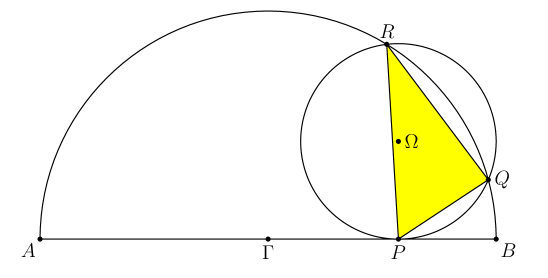
\includegraphics[scale=0.5]{Geometry}
    \end{figure}
\end{frame}

\begin{frame}{Solution 1}
    \begin{columns}    
        \column{0.5\textwidth}
        \begin{figure}[h]
            \centering
            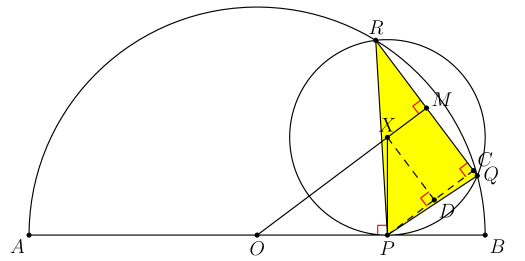
\includegraphics[scale=0.3]{Geometry Solution 1.PNG}
            \captionsetup{labelformat=empty}
            \caption{Solution 1: Find the height $PC$}
        \end{figure}

        \column{0.5\textwidth}
        To find out $a+b+c$, we need to find the area of $\triangle PQR$.
        Since we have know $QR = 3\sqrt{3}$, it suffices to find $PC$, which is the height based on $QR$.
        \pause

        As shown in the graph, to find out $PC$, we can find $PD$ and $DC$ first and then add them up.
        Also, $DC = XM$ since $DCMX$ is a rectangle.
    \end{columns}
\end{frame}

\begin{frame}{}
    \begin{columns}    
        \column{0.5\textwidth}
        \begin{figure}[h]
            \centering
            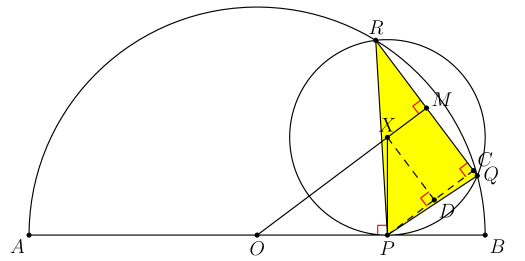
\includegraphics[scale=0.3]{Geometry Solution 1.PNG}
            \captionsetup{labelformat=empty}
            \caption{Solution 1: Find the height $PC$}
        \end{figure}

        \column{0.5\textwidth}
        To find $XM$, notice that it is the height of $\triangle RXQ$ based on $RQ$.
        By the Law of Sine, we know the radius $XP$ of circle $X$ is
        \[
            XP = \frac{QR}{2\sin\angle QPR} = \frac{3\sqrt{3}}{2 \cdot \frac{\sqrt{3}}{2}} = 3.
        \]
        \pause
        By the Inscribed Angle Theorem, $\angle QXR = 2 \angle QPR = 120^\circ$, so $\triangle QXR$ is an isosceles triangle with angles $120^\circ, 30^\circ, 30^\circ$.
        \pause
        
        Thus, $DC = XM = RX \sin 30^\circ = \frac{3}{2}$.
    \end{columns}
\end{frame}

\begin{frame}{}
    \begin{columns}    
        \column{0.5\textwidth}
        \begin{figure}[h]
            \centering
            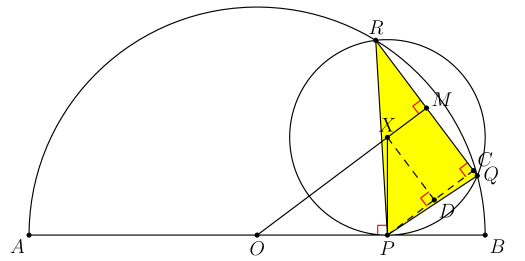
\includegraphics[scale=0.3]{Geometry Solution 1.PNG}
            \captionsetup{labelformat=empty}
            \caption{Solution 1: Find the height $PC$}
        \end{figure}

        \column{0.5\textwidth}
        Now let's find $PD$.
        \pause
        Notice that $\triangle PDX$ is a right triangle similar to $\triangle XPO$ since $\angle DPX$ and $\angle PXO$ are alternate interior angles.
        \pause
        So, we have the relation
        \[
            \frac{PD}{XP} = \frac{XP}{OX}.
        \]
    \end{columns}
\end{frame}

\begin{frame}{}
    \begin{columns}    
        \column{0.5\textwidth}
        \begin{figure}[h]
            \centering
            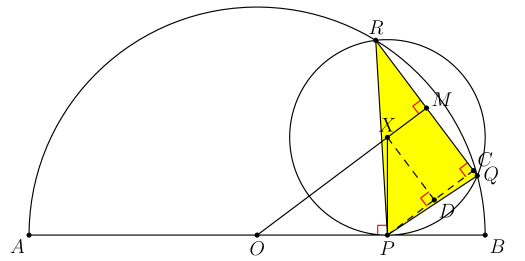
\includegraphics[scale=0.3]{Geometry Solution 1.PNG}
            \captionsetup{labelformat=empty}
            \caption{Solution 1: Find the height $PC$}
        \end{figure}

        \column{0.5\textwidth}
        We know $XP = 3$.
        %If we can find $OP$, then we can solve $PD$.
        %\pause
        %Since $\triangle OPX$ is a right triangle, we can find $OX$ first, then use Pythagorean Theorem to calculate $OP$.
        %\pause
        Notice that $\triangle OMR$ is a right triangle with $OR = 7$ and $\displaystyle RM = \frac{3\sqrt{3}}{2}$.
        By Pythagorean Theorem we have $\displaystyle OM = \sqrt{OR^2-RM^2} = \frac{13}{2}$, so $OX = OM-XM = 5$.
        \pause
        Using Pythagorean Theorem again, we get $\displaystyle OP = \sqrt{OX^2-XP^2} = 4$, thus
        \[
            PD = XP \cdot \frac{XP}{OX} = \frac{9}{5}.
        \]
    \end{columns}
\end{frame}

\begin{frame}{}
    \begin{columns}    
        \column{0.5\textwidth}
        \begin{figure}[h]
            \centering
            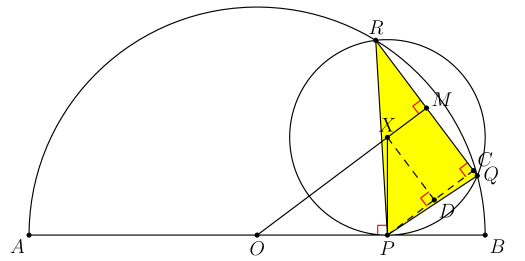
\includegraphics[scale=0.3]{Geometry Solution 1.PNG}
            \captionsetup{labelformat=empty}
            \caption{Solution 1: Find the height $PC$}
        \end{figure}

        \column{0.5\textwidth}
        Finally, we have
        \[
            PC = PD+DC = \frac{9}{5}+\frac{3}{2} = \frac{33}{10},
        \]
        \pause
        and the area
        \[
            \frac{1}{2} \cdot QR \cdot PC = \frac{99\sqrt{3}}{20}.
        \]
        \pause
        Therefore $a = 99$, $b = 3$, $c = 20$, and $a+b+c = 122$.
    \end{columns}
\end{frame}

\begin{frame}{Reflection}
    Here are some tips for this type of questions.
    \begin{itemize}
        \item If you can directly find $a+b+c$, do it.

        \item If you decide to find out the area, determine a method and stick to it.

        \item Make proper auxiliary lines to help, not to mess up.
    \end{itemize}
\end{frame}

\begin{frame}{}
    \begin{figure}[h]
        \centering
        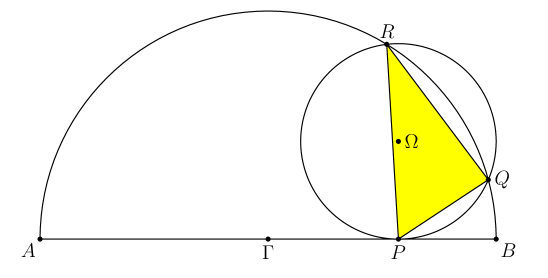
\includegraphics[scale=0.5]{Geometry.PNG}
        \captionsetup{labelformat=empty}
        \caption{Solution 2?}
    \end{figure}
\end{frame}

\section{Demo 09/13/24}

\begin{frame}{Polynomials}
    $f(x) = 2x^2+3x+4$, $g(x) = x^3-5x+6$, and $h(x) = 4x^4+3x^3+2x^2+1$ are polynomials.\pause

    The general form for a \emph{polynomial} with degree $n$ is
    \[
        p(x) = a_nx^n+a_{n-1}x^{n-1}+a_{n-2}x^{n-2} + \cdots + a_1x+a_0,
    \]
    where $a_i$'s are \emph{coefficients} of powers of $x$ and $a_n \neq 0$, $a_n$ is called \emph{leading coefficient}, and the degree of the polynomial is the value $n$.
\end{frame}

\begin{frame}{Polynomial Divisions}
    Let $p(x)$ and $g(x)$ be polynomials with $deg(g(x)) < deg(p(x))$, then there exist unique polynomials $q(x)$ and $r(x)$ such that
    \[
        p(x) = g(x) \cdot q(x) + r(x),
    \]
    where the degree of $r(x)$ satisfies $0 \leq deg(r(x)) < deg(g(x))$.\pause

    $q(x)$ is called the \emph{quotient polynomial} and $r(x)$ is called the \emph{remainder polynomial}.

    \note{Give examples to show the items, and compare the polynomial divisions with the integer divisions.}
\end{frame}

\begin{frame}{Remainder Theorem}
    When $p(x)$ is divided by a polynomial of degree $n$, the remainder can be assumed to be of the degree $n-1$.\pause

    \note{Example to illustrate.}

    When the polynomial $p(x)$ is divided by $(ax-b)$, if we set $x = \frac{b}{a}$, then we can find the remainder is $p(\frac{b}{a})$:
    \[
        p(x) = (ax-b)q(x)+r \Rightarrow p(\frac{b}{a}) = r.
    \]
    \pause
\end{frame}

\begin{frame}{Problem 1}
    Find the remainder when $x^{100}+1$ is divided by $x-1$.
\end{frame}

\begin{frame}{Problem 2}
    Find the remainder when $x^{100}-2x^{51}+1$ is divided by $x^2-1$.
\end{frame}

\begin{frame}{Factor Theorem}
    $c$ is a root of a polynomial $p(x)$, i.e., $p(c) = 0$, iff $(x-c)$ is a factor of $p(x)$, i.e., there exists $q(x)$ such that $p(x) = (x-c) \cdot q(x)$.\pause

    Ex. Is $(x-2)$ a factor of $p(x) = x^3+x^2+x-14$?
\end{frame}

\begin{frame}{Vieta's Theorem}
    If $x_1$ and $x_2$ are the two roots of $ax^2+bx+c=0$ where $a \neq 0$, then
    \[
        x_1+x_2 = -\frac{b}{a}, x_1 \cdot x_2 = \frac{c}{a}.
    \]
    \pause
    
    If $x_1$, $x_2$, and $x_3$ are the three roots of $ax^3+bx^2+cx+d=0$ where $a \neq 0$, then
    \[
        x_1+x_2+x_3 = -\frac{b}{a}, x_1 \cdot x_2 + x_1 \cdot x_3 + x_2 \cdot x_3 = \frac{c}{a}, x_1 \cdot x_2 \cdot x_3 = -\frac{d}{a}.
    \]
    \pause

    \note{Give examples for quadratic and cubic cases, and show how to deduce the equations.}
\end{frame}

\begin{frame}{}
    If $x_1$, $x_2$, $\dots$, and $x_n$ are the $n$ roots of $n$-th polynomial equation
    \[
        a_n x^n + a_{n-1} x^{n-1} + \cdots + a_1 x + a_0 = 0,
    \]

    then
    \begin{align*}
        & \sum_{i=1}^n x_i = -\frac{a_{n-1}}{a_n},\\
        & \sum_{1 \leq i < j \leq n} x_i x_j = \frac{a_{n-2}}{a_n},\\
        & \dots\\
        & \sum_{1 \leq i_1 < i_2 < \cdots < i_k \leq n} x_{i_1} x_{i_2} \cdots x_{i_k} = (-1)^k \frac{a_{n-k}}{a_n},\\
        & \dots\\
        & \prod_{i=1}^n x_i = (-1)^n \frac{a_0}{a_n}.
    \end{align*}
\end{frame}

\begin{frame}{Problem 3}
    Find $a$ and $b$ if $f(x) = x^4-5x^3+11x^2+ax+b$ is divisible by $g(x) = (x-1)^2$.
\end{frame}

\end{document} 
